\section{Bounds from partial observations}
\label{sec:bounds}

A shift total can bound the hours worked before a release even when the start time is unknown. If one person spent $v$ hours on a task across two periods lasting $b$ and $c$ hours, the amount $x$ in the first period satisfies
\[
  \max(0,v-c)\le x\le\min(v,b).
\]
Any hours that exceed the capacity of the second period must fall in the first. The upper limit is the smaller of the task total and the duration of that first period.

Suppose an engineer spent one hour implementing a feature and one hour repairing a defect within a two-hour shift. Each activity can fill the first hour in a different schedule, as Figure~\ref{fig:shared-time} shows. Adding their separate maxima would assign two person-hours to an engineer with one hour available. The second hour can absorb at most one person-hour of the two-hour total. Exactly one person-hour therefore falls in the first hour.

\begin{figure}[ht]
\centering
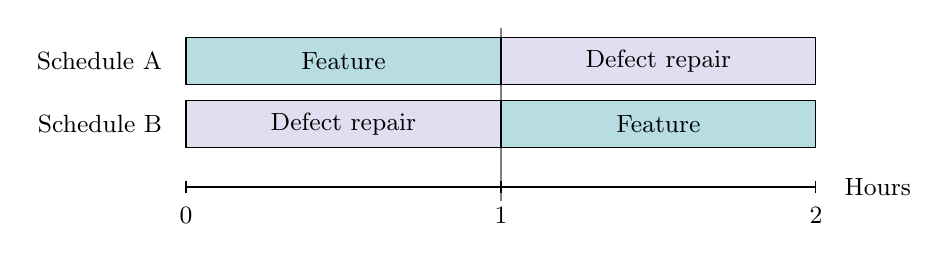
\begin{tikzpicture}[x=4.0cm,y=.8cm,font=\small]
  \definecolor{feature}{HTML}{B7DDE3}
  \definecolor{repair}{HTML}{E1DEF1}
  \draw[gray] (1,.15) -- (1,2.9);
  \draw[fill=feature] (0,2) rectangle (1,2.75);
  \draw[fill=repair] (1,2) rectangle (2,2.75);
  \draw[fill=repair] (0,1) rectangle (1,1.75);
  \draw[fill=feature] (1,1) rectangle (2,1.75);
  \node[anchor=east] at (-.045,2.375) {Schedule A};
  \node[anchor=east] at (-.045,1.375) {Schedule B};
  \node at (.5,2.375) {Feature};
  \node at (1.5,2.375) {Defect repair};
  \node at (.5,1.375) {Defect repair};
  \node at (1.5,1.375) {Feature};
  \draw (0,.38) -- (2,.38);
  \foreach \x in {0,1,2} {
    \draw (\x,.28) -- (\x,.48);
    \node[below=1.5pt] at (\x,.28) {\x};
  }
  \node[anchor=west] at (2.06,.38) {Hours};
\end{tikzpicture}
\caption{Two schedules consistent with one hour of feature work and one hour of repair by the same engineer. The first hour contains one person-hour in either schedule.}
\label{fig:shared-time}
\end{figure}


\subsection{Compute the range on a shared time axis}

Use $g$ to denote one contributor's activity on one task and $j(g)$ for that contributor. Cover the full span of each observation, including work outside the target when it shares an observed total with work in scope. Partition the time axis at every observation boundary and every target boundary. Each resulting cell $J_k$ has duration $d_k>0$ in hours. Let $x_{gk}$ be the person-hours of activity $g$ in cell $k$.

An observation $\nu$ supplies a range $[v^-_\nu,v^+_\nu]$ for the combined hours of activities $G_\nu$ during a set $K_\nu$ of whole cells. An exact measurement sets both endpoints equal. Widen the interval to allow for rounding or other known error. The arrays $x$ must satisfy
\begin{align}
 x_{gk} &\ge 0, &
 \sum_{g:j(g)=j}x_{gk} &\le d_k,\\
 v^-_\nu &\le \sum_{g\in G_\nu}\sum_{k\in K_\nu}x_{gk}
 \le v^+_\nu.
\end{align}
Nonnegativity holds for each activity in each cell. Apply the capacity limit to each contributor in each cell and the observation limit to every $\nu$. To represent an absence, cut at its boundaries and set that contributor's hours to zero in the affected cells.

Write $\mathcal P$ for the set of arrays satisfying the constraints. Sum the target hours as $h(x)=\sum_{g,k}w_{gk}x_{gk}$, with $w_{gk}=1$ for work in scope and $0$ elsewhere. If $\mathcal P$ is nonempty, solve two linear programmes to obtain
\begin{equation}
  [L,U]=\left[\min_{x\in\mathcal P}h(x),\,
                    \max_{x\in\mathcal P}h(x)\right].
  \label{eq:labour-bounds}
\end{equation}
Integrating any allocation that satisfies the observation and time limits yields an array in $\mathcal P$. The corresponding total therefore lies in $[L,U]$. An empty $\mathcal P$ means that the supplied limits are inconsistent under the accounting rules.

\subsection{When the endpoints can occur}

The cell model recovers exactly the possible totals when people can divide their time among eligible activities within each cell. One allocation uses a constant share $x_{gk}/d_k$ for every activity in that cell. If each person must work on one activity at a time, schedule each activity in one block of length $x_{gk}$ and leave any remaining time idle. One block per activity per cell suffices to recover the observations and the target total. The feasible set is closed and bounded, so both extrema exist. A weighted average of the two optimising arrays preserves all constraints and realises the corresponding intermediate total. The allocation argument applies to that array as well.

A minimum session length or fixed activity order can rule out some of these allocations. Equation~\eqref{eq:labour-bounds} still encloses every total that satisfies the added scheduling rules. The endpoints are tight if each occurs under those rules. Suppose an uninterrupted one-hour session must fit into one of two one-hour periods separated by an absence. The session contributes a full hour to whichever period contains it, so the first-period total can be zero or one hour.

A rule requiring two people to review together can enter the linear programme directly. Suppose a finite set of working configurations describes the combinations allowed at each instant. A configuration specifies each person’s activity or idle time. For paired review, the permitted configurations put both named reviewers on the review whenever either is reviewing. Allocate a nonnegative duration to each permitted configuration. Require their durations to sum to $d_k$. Then $x_{gk}$ is the sum of durations for configurations containing $g$. Each permissible allocation supplies the duration spent in each configuration. If the team can switch configurations within the cell, consecutive blocks of those lengths recover the observed totals.

\subsection{When the observations leave work uncovered}

If $[L,U]$ covers the included contributors' hours and an independent check caps uncounted hours at $B$, the combined total lies in $[L,U+B]$. When the extra hours have no established upper limit, restrict the conclusion to $[L,U]$ for the included contributors. For observations from a sample, the target range covers the true total whenever all observation ranges cover their respective values and the true allocation satisfies the capacity constraints. By the union bound, observation ranges with failure probabilities summing to at most $\alpha$ give target coverage of at least $1-\alpha$ even when the observations depend on one another.
